\documentclass[11pt,notes=hide,aspectratio=169,mathserif]{beamer}

% PACKAGES
\usepackage{graphics}  % Support for images/figures
\usepackage{graphicx}  % Includes the \resizebox command
\usepackage{tikz}      % For flowcharts
\usetikzlibrary{arrows.meta, positioning} % Libraries for TikZ


\usepackage{url}	   % Includes \urldef and \url commands
\usepackage{natbib}
\usepackage{bibentry}  % Includes the \nobibliography command
\usepackage{verbatim}  %Supports comments
\usepackage{booktabs} %Supports \toprule, \bottomrule, etc in tables
\usepackage{etoolbox}  %Supports toggle commands
\usepackage{datetime}
\usepackage{bm}	%Supports bold math \bm
%the LaTeX standard:
\usepackage{cmbright}
\setbeamerfont{frametitle}{family=\fontfamily{cmbr}\selectfont,size=\Large}
\fontencoding{OT1}\fontfamily{cmbr}\selectfont

% PACKAGES (that should already be included by your LyX document settings)
\usepackage{amsfonts}  % Lots of stuff, including \mathbb 
\usepackage{amsmath}   % Standard math package
\usepackage{amsthm}    % Includes the comment functions
\usepackage{subcaption}

% CUSTOM DEFINITIONS
\def\newblock{} %Get beamer to cooperate with BibTeX
\linespread{1.2}

% IDENTIFYING INFORMATION
\title[class]{ECON 326: Economics of Developing Countries \\ TA Session 2}
\author[vaidehi's class ]{Vaidehi Parameswaran (Northwestern Econ)}
\date{\monthname[\the\month] \the\year}

% THEMATIC OPTIONS
%\setbeamercovered{transparent}
\usetheme{metropolis}
\definecolor{mycolor}{RGB}{0,153,153} % define cyan colour
\setbeamercolor{frametitle}{bg=mycolor, fg=white} % Frame title color
\setbeamercolor{title separator}{fg=mycolor} 
\setbeamercolor{progress bar}{fg=mycolor} 
\beamertemplatenavigationsymbolsempty
\setbeamertemplate{footline}[frame number]{}
\setbeamertemplate{itemize item}{\small\raisebox{1pt}{\textcolor{mycolor}{$\blacktriangleright$}}}
\setbeamertemplate{itemize subitem}{\footnotesize\raisebox{1pt}{\textcolor{mycolor}{$\triangleright$}}}
\setbeamertemplate{itemize subsubitem}{\tiny\raisebox{1pt}{\textcolor{mycolor}{$\triangleright$}}}

% BACKUP SLIDE NUMBERING
\usepackage{appendixnumberbeamer}

\begin{document}

%---------------------------------------------------------------------
\begin{frame}[plain]
\titlepage
\end{frame}
%---------------------------------------------------------------------

%\section{Overview}

%---------------------------------------------------------------------
\begin{frame}{Today's Agenda}
\begin{itemize}
\item Interaction Terms
\item IV Application: Acemoglu, Johnson, and Robinson (2001)
\item Stata: \texttt{merge}, \texttt{reshape}
\end{itemize}
\end{frame}
%---------------------------------------------------------------------


\section*{Interactions}

%---------------------------------------------------------------------
\begin{frame}{Interaction Terms}
\begin{itemize}
\item Ignore endogeneity concerns for now 
\item Consider the following estimating equation:
\begin{equation}
\label{eq:1}
    Y_i = \alpha + \beta X_i + \epsilon_i
\end{equation}
\item If treatment effects are heterogeneous across observations, we want $\beta$ to be indexed by $i$. 
\item Estimating equation \eqref{eq:1} yields the \textbf{average effect} of $X$ on $Y$.
\item Suppose we want to control for the effect of $W$ on $Y$.
\item We can include an interaction term between $X$ and $W$ in the estimating equation:
\begin{equation}
\label{eq:2}
    Y_i = \alpha + \beta X_i + \gamma W_i + \delta (X_i \times W_i) + \epsilon_i
\end{equation}
\end{itemize}
\end{frame}
%---------------------------------------------------------------------

%---------------------------------------------------------------------
\begin{frame}{Interaction Terms}
\begin{itemize}
\item Take conditional expectations of $Y$ given $X$ and $W$:
\begin{equation}
\label{eq:3}
    E[Y_i|X_i,W_i] = \alpha + \beta X_i + \gamma W_i + \delta (X_i \times W_i)
\end{equation}
\item So now the effect of $X$ on $Y$ is $\beta + \delta W_i$.
\item If $X$ is continuous, 
\begin{equation}
\label{eq:4}
    \frac{\partial E[Y_i|X_i,W_i]}{\partial X_i} = \beta + \delta W_i
\end{equation}
\item If $X$ is binary,
\begin{equation}
\label{eq:5}
    E[Y_i|X_i=1,W_i] - E[Y_i|X_i=0,W_i] = \beta + \delta W_i
\end{equation}
\end{itemize}
\end{frame}
%---------------------------------------------------------------------

%---------------------------------------------------------------------
\begin{frame}{Interaction Terms}
\begin{itemize}
\item Reading a table:
\begin{figure}
\centering
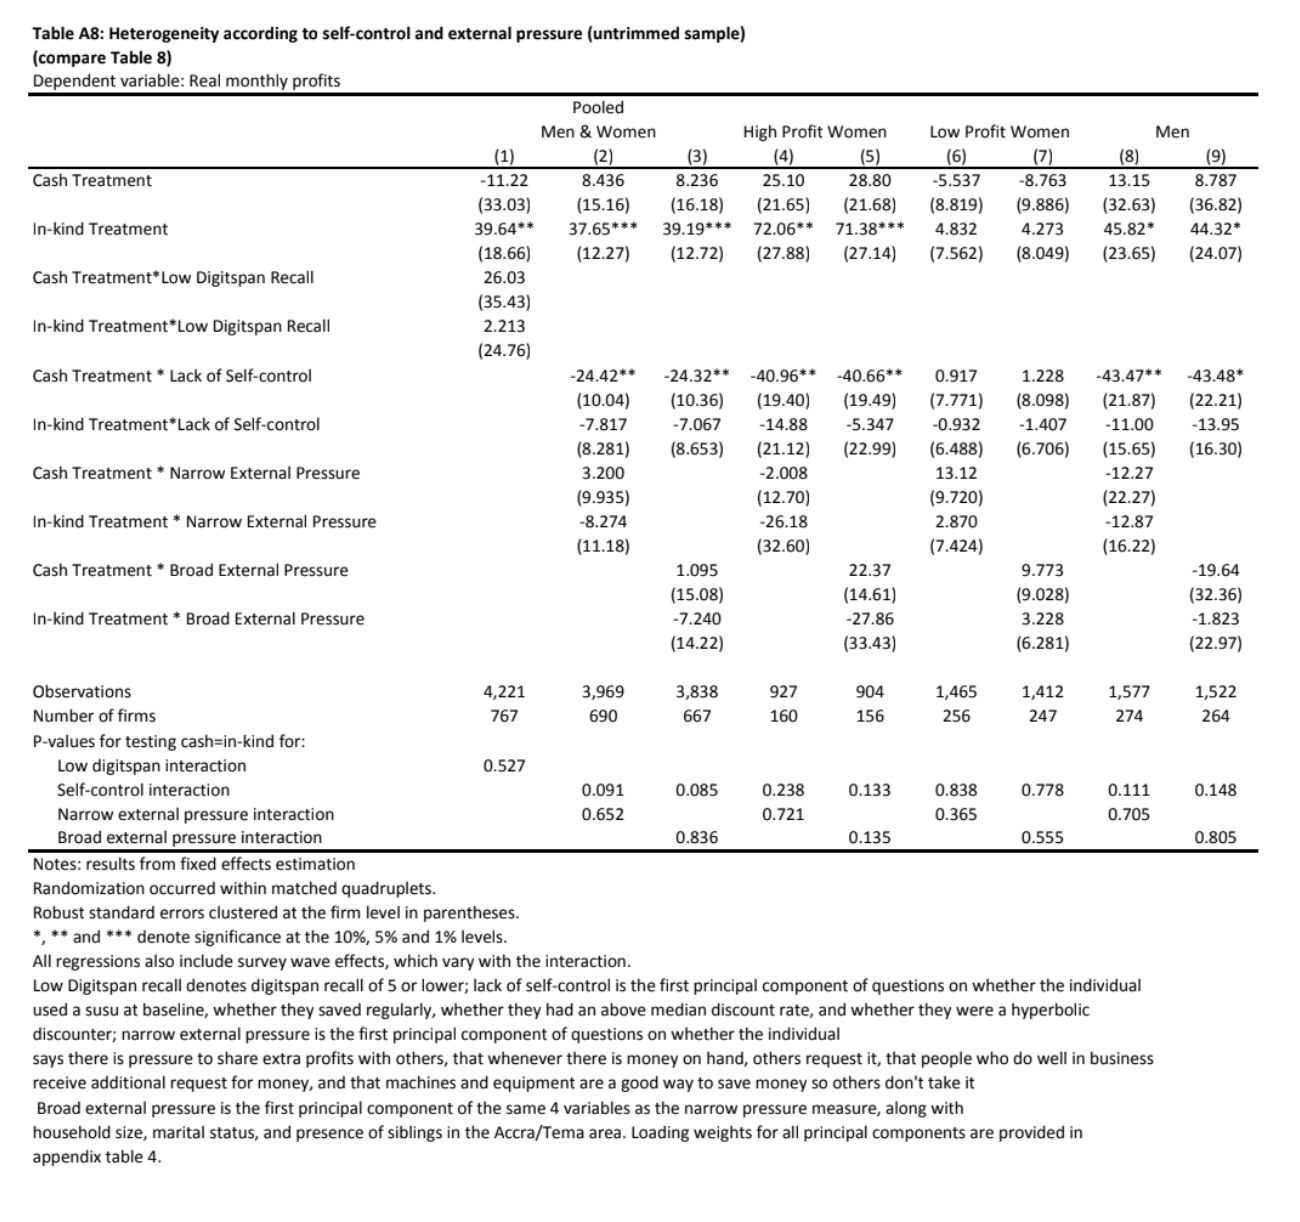
\includegraphics[width=0.7\textwidth]{inputs/interactions.png}
\caption{Source: Fafchamps et al. (2013)}
\end{figure}
\end{itemize}
\end{frame}
%---------------------------------------------------------------------

\section*{IV Application  - AJR (2001)}
%---------------------------------------------------------------------
\begin{frame}{Institutions and Development}
\begin{itemize}
\item Institutions: set the ``rules of the game'' in a society
\item So agents have to make decisions under these constraints
\item Intuitive that having good institutions is better for development
\item But causality is hard to establish
\end{itemize}
\end{frame}
%---------------------------------------------------------------------

%---------------------------------------------------------------------
\begin{frame}{AJR (2001): Measurement of Institutions}
\begin{itemize}
\item Institution quality measured as an index of protection against expropriation risk
\item Constructed from political risk rating agencies
\item Issues: subjective, volatile 
\end{itemize}
\end{frame}
%---------------------------------------------------------------------

%---------------------------------------------------------------------
\begin{frame}{AJR (2001): Correlation}
\begin{itemize}
\item Consider the regression of GDP per capita on institutional quality
\begin{figure}
\centering
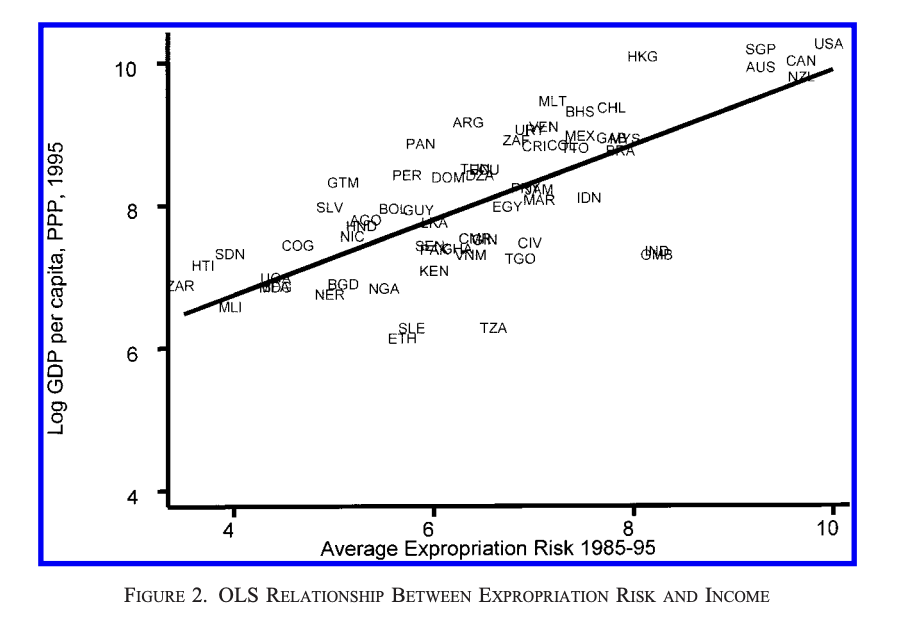
\includegraphics[width=0.7\textwidth]{inputs/AJR1.png}
\caption{Source: Acemoglu, Johnson, and Robinson (2001)}
\end{figure}
\item Strong, positive correlation
\end{itemize}
\end{frame}
%---------------------------------------------------------------------

%---------------------------------------------------------------------
\begin{frame}{AJR (2001): Correlation}
\begin{itemize}
\item But ... is it causal? 
\begin{itemize}
    \item Reverse causality?
    \item Omitted variable bias?
\end{itemize}
\item Strategy: Instrumental Variables (IVs)
\item Recall the conditions for the IV to be appropriate:
\begin{itemize}
    \item Relevance: $Cov(Z, X) \neq 0$
    \item Exogeneity: $\mathbb{E}(Z, \epsilon) = 0$
\end{itemize}
\end{itemize}
\end{frame}
%---------------------------------------------------------------------

%---------------------------------------------------------------------
\begin{frame}{AJR (2001): IV}
\begin{itemize}
\item AJR use \textbf{settler mortality}
\begin{itemize}
    \item Relevance? Extractive institutions vs inclusive institutions
    \item Exogeneity? Plausibly governed by geographical factors that are no longer relevant to GDP today
\end{itemize}
\item We see some of these institutional differences even today
\end{itemize}
\end{frame}
%---------------------------------------------------------------------

%---------------------------------------------------------------------
\begin{frame}{AJR (2001): IV}
\begin{center}
    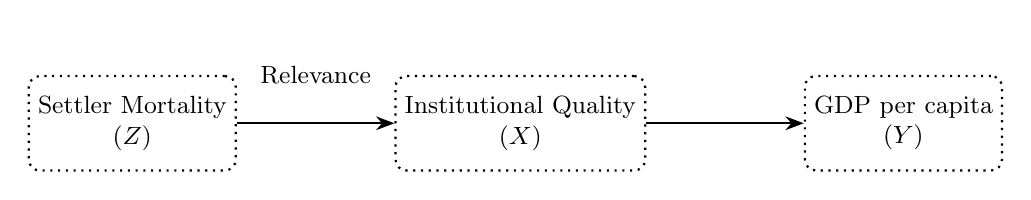
\begin{tikzpicture}[
        node distance=2.5cm and 2cm,
        every node/.style={draw, dotted,rounded corners, minimum width=2.5cm, minimum height=1.2cm, align=center, font=\small},
        every path/.style={-Stealth, thick}
    ]
    
    % Nodes
    \node (Z) {Settler Mortality \\ (\( Z \))};
    \node[right=of Z] (X) {Institutional Quality \\ (\( X \))};
    \node[right=of X] (Y) {GDP per capita \\ (\( Y \))};
    
    % Arrows
    \draw (Z) -- (X) node[midway, above, draw=none] {Relevance};
    \draw (X) -- (Y) ; 
    
    \end{tikzpicture}
    \end{center}
\begin{itemize}
    \item We want to say X causes Y
    \item But we have endogeneity
    \item As an IV, we want Z to affect X 
    \item And we want Z to affect Y but only through X
\end{itemize}
\end{frame}
%---------------------------------------------------------------------

%---------------------------------------------------------------------
\begin{frame}{AJR (2001): Results}
\begin{itemize}
\item First-stage result
\begin{figure}
\centering
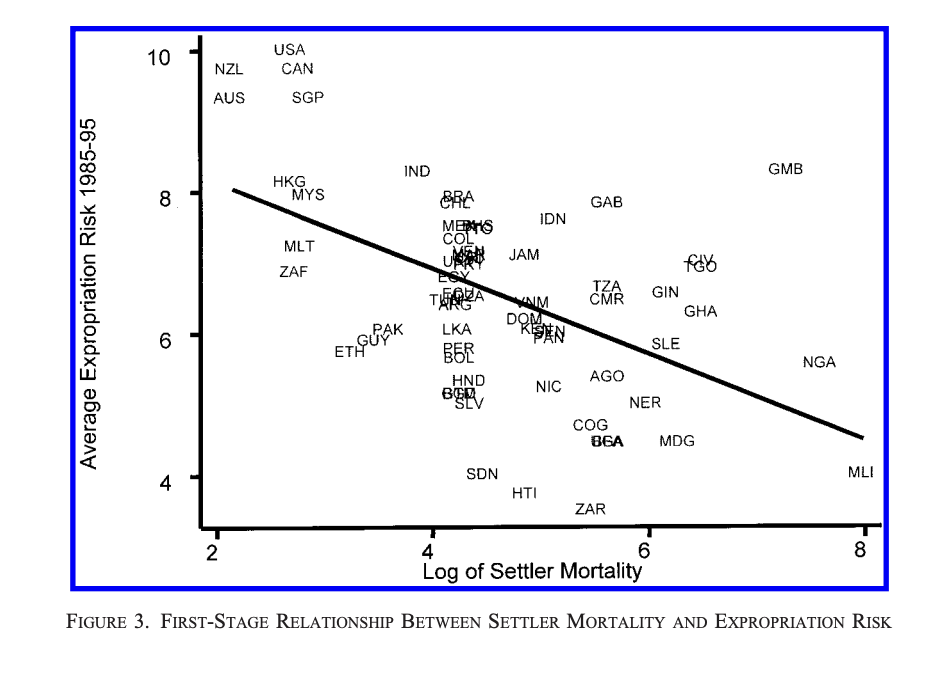
\includegraphics[width=0.7\textwidth]{inputs/AJR2.png}
\caption{Source: Acemoglu, Johnson, and Robinson (2001)}
\end{figure}
\item $Z$ is negatively correlated with $X$
\end{itemize}
\end{frame}
%---------------------------------------------------------------------

%---------------------------------------------------------------------
\begin{frame}{AJR (2001): Results}
\begin{itemize}
\item Reduced form
\begin{figure}
\centering
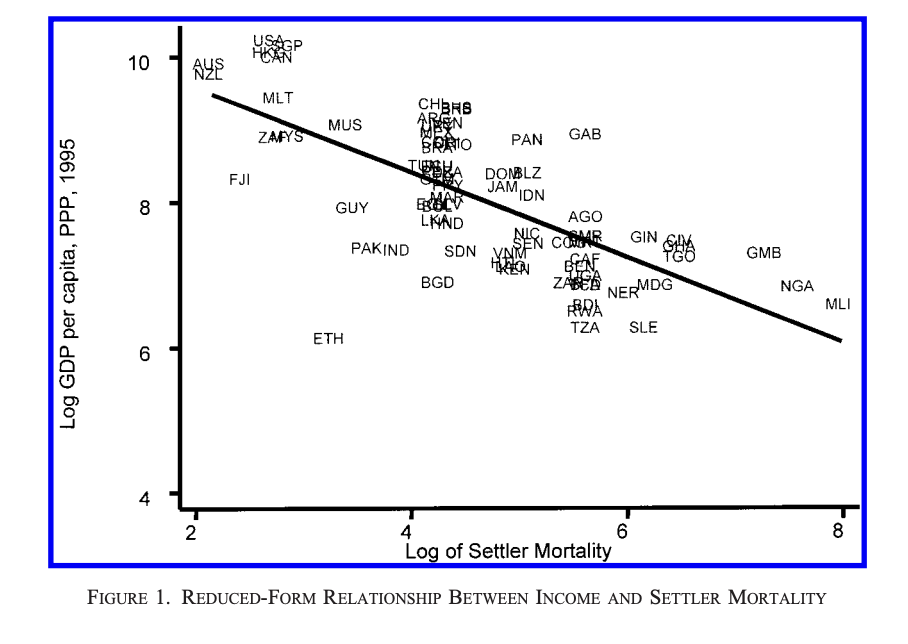
\includegraphics[width=0.7\textwidth]{inputs/AJR3.png}
\caption{Source: Acemoglu, Johnson, and Robinson (2001)}
\end{figure}
\item Under conditions of relevance and exogeneity, higher settler mortality drives lower GDP per capita. 
\end{itemize}
\end{frame}
%---------------------------------------------------------------------

%---------------------------------------------------------------------
\begin{frame}{AJR (2001): Results}
\begin{itemize}
\item IV estimates:
\begin{figure}
\centering
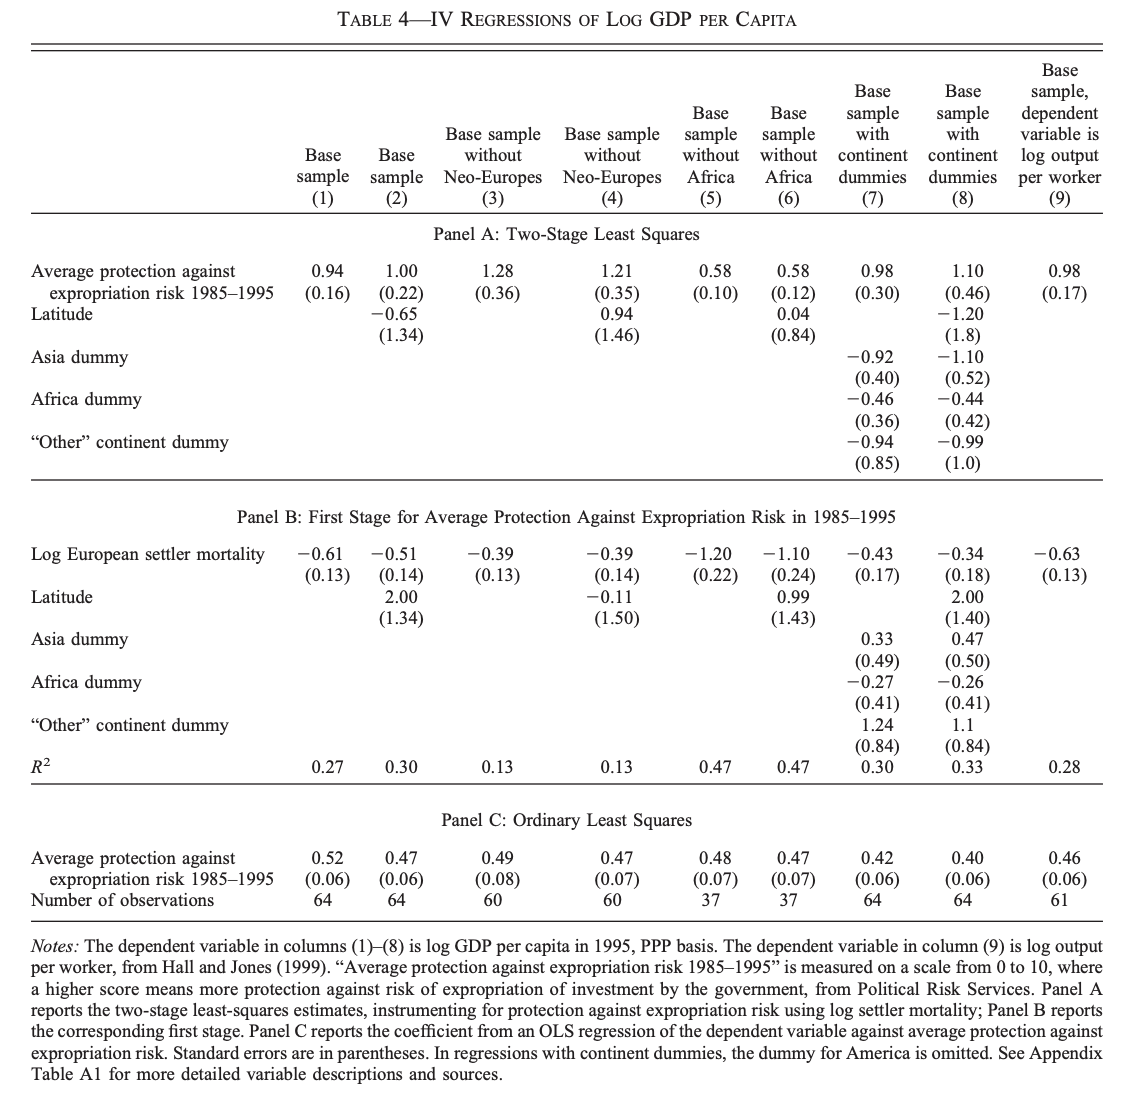
\includegraphics[width=0.4\textwidth]{inputs/AJR4.png}
\caption{Source: Acemoglu, Johnson, and Robinson (2001)}
\end{figure}
\end{itemize}
\end{frame}
%---------------------------------------------------------------------

%---------------------------------------------------------------------
\begin{frame}{Glaeser's Critique}
\begin{itemize}
\item Glaeser et al. (2004) argue that:
\begin{enumerate}
    \item Institutions are mismeasured
    \item Z is correlated with Y through human capital, so exogeneity fails
\end{enumerate}
\item GLLS propose human capital as an explanation for cross-country income differences
\end{itemize}
\end{frame}
%---------------------------------------------------------------------

    
%---------------------------------------------------------------------
\begin{frame}{Issue 1: Measurement}
\begin{itemize}
\item Subjective measure of quality which could be affected by GDP itself
\begin{itemize}
    \item Richer countries may have higher ratings 
\end{itemize}
\item The index reflects outcomes
\begin{itemize}
    \item The index is lower in countries where expropriations have happened
    \item But expropriations themselves are a function of the constraints and a choice variable
    \item Two countries with the same set of constraints may have different outcomes because of different choices by leaders
\end{itemize}
\end{itemize}
\end{frame}
%---------------------------------------------------------------------

%---------------------------------------------------------------------
\begin{frame}{Issue 2: Exogeneity}
\begin{itemize}
\item AJR's key idea: \textit<overlay specification>{if Europeans want to settle somewhere, they bring good institutions}
\item But they could have also brought with them good human capital
\item So settler mortality and human capital maybe correlated
\item Human capital could affect today's GDP
\item Thus the instrument $Z$ affects $Y$ through the channel of human capital, not just $X$
\item This is a violation of the exclusion restriction
\item And thus a threat to identification
\end{itemize}
\end{frame}
%---------------------------------------------------------------------

%---------------------------------------------------------------------
\begin{frame}{GLLS (2004)}
\begin{itemize}
\item AJR's IV can predict human capital since the 1900s
\begin{figure}
\centering
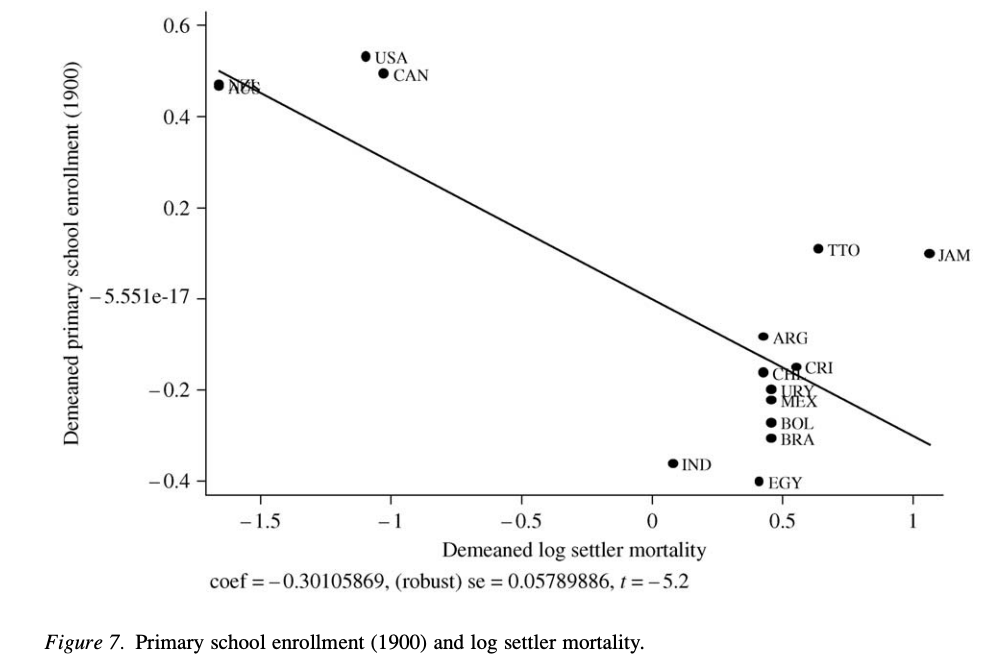
\includegraphics[width=0.7\textwidth]{inputs/GLLS1.png}
\caption{Source: Glaeser et al. (2004)}
\end{figure}
\end{itemize}
\end{frame}
%---------------------------------------------------------------------

%---------------------------------------------------------------------
\begin{frame}{GLLS (2004)}
\begin{itemize}
\item So which is it? How can we square AJR and GLLS?
\item Do institutions cause growth? 
\item Does human capital cause growth?
\item Or is it both?
\item GLLS attempt to identify the effects of both channels 
\item They find that human capital is a source of growth rather than institutions
\end{itemize}
\end{frame}
%---------------------------------------------------------------------

\section*{Stata}

%--------------------------------------------------------------------- 
\begin{frame}{Stata: \texttt{merge}}
\begin{itemize}
\item Merging datasets is probably one of the most common tasks in data management
\item And it's one thing Stata does easily and well
\item Why merge? Typically to bring in additional variables
\item What you need? 2 datasets and a common identifier variable in both
\item The command: \texttt{merge TYPE IDVAR using filename}
\item Example: \texttt{merge 1:1 id using filename}
\end{itemize}
\end{frame}
%---------------------------------------------------------------------

%--------------------------------------------------------------------- 
\begin{frame}{Stata: \texttt{merge}}
\begin{itemize}
\item Types of merges:
\begin{itemize}
    \item \texttt{1:1}: Unique identifier in both datasets
    \item \texttt{1:m}: A merge where the first dataset has one observation for each unique identifier, and the second dataset has multiple observations for each unique identifier
    \item \texttt{m:1}: The opposite of \texttt{1:m}
    \item \texttt{m:m}: You NEVER want to do this
\end{itemize}
\item Make sure the merging variable has the same name in both datasets
\item It's also good practice to make sure it has the same variable type 
\end{itemize}
\end{frame}
%---------------------------------------------------------------------

%--------------------------------------------------------------------- 
\begin{frame}{Stata: \texttt{merge}}
\begin{itemize}
\item Reading merge results:
\end{itemize}
\end{frame}
%---------------------------------------------------------------------
    

%--------------------------------------------------------------------- 
\begin{frame}{Stata: \texttt{reshape}}
\begin{itemize}
\item Suppose you have a dataset with variable $X_ij$
\item So say $i$ is the individual and $j$ is the year, and $X$ is income 
\item Such a dataset can be stored in two different formats in Stata:
\begin{itemize}
    \item Wide format: Each individual has a row and each year has a column
    \item Long format: Each individual-year pair has a row
\end{itemize}
\end{itemize}
\end{frame}
%---------------------------------------------------------------------

%--------------------------------------------------------------------- 
\begin{frame}{Stata: \texttt{reshape}}
\begin{itemize}
\item What it looks like:
\end{itemize}
\begin{figure}[htbp]
\centering
\begin{subfigure}{0.25\textwidth}
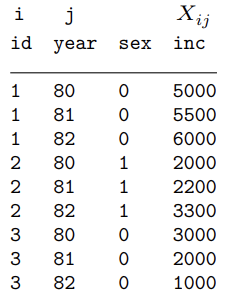
\includegraphics[width=\textwidth]{inputs/reshape1.png}
\caption{Long format}
\end{subfigure}
\hfill
\begin{subfigure}{0.45\textwidth}
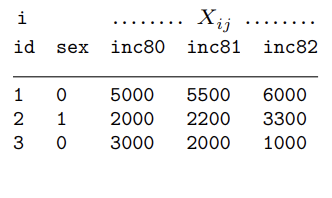
\includegraphics[width=\textwidth]{inputs/reshape2.png}
\caption{Wide format}
\end{subfigure}
\end{figure}
\end{frame}
%---------------------------------------------------------------------
    
%--------------------------------------------------------------------- 
\begin{frame}{Stata: \texttt{reshape}}
\begin{itemize}
\item To reshape from long to wide, use the command \texttt{reshape wide \textit{varlist}, i(i) j(j) }
\begin{itemize}
    \item $i$ is the identifier variable
    \item $j$ is the variable that will be spread out (in this case, year)
    \item \textit{varlist} is the list of variables that will be spread out
    \item you need to include all the variables that vary at the $i-j$ level in your  \textit{varlist}
\end{itemize}

\item To reshape from wide to long, use the command \texttt{reshape long \textit{varlist}, i(i) j(j) }
\begin{itemize}
    \item $i$ is the identifier variable
    \item $j$ is a new variable that will be created (in this case, year) 
    \item \textit{varlist} is the variable prefix ($inc$ in this case)
\end{itemize}
\item Since \texttt{sex} is common within $i$, it doesn't need to be included in the \textit{varlist}
\end{itemize}
\end{frame}
%---------------------------------------------------------------------


%---------------------------------------------------------------------
\begin{frame}
\begin{center}{\LARGE See you next time!}\end{center}
\end{frame}
%---------------------------------------------------------------------


\end{document}